\documentclass[11pt]{article}

\usepackage{/home/paul/Workspace/build/macros}


\usepackage{geometry}
\geometry{margin=0.9in}
\geometry{letterpaper}    
\usepackage{graphicx}

\usepackage{subfig}


\usepackage[francais]{babel}

\usepackage{matlab-prettifier}
\usepackage{listings}
\lstset{
	style = Matlab-editor,
	breaklines = true,
	basicstyle = \footnotesize\ttfamily,
	extendedchars = true,
	frame = single
}

\usepackage{fancyhdr}
\pagestyle{fancy}
\fancyhead{}

\usepackage[style=alphabetic]{biblatex}
%\usepackage[backend=biber,style=alphabetic]{biblatex}
\bibliography{/home/paul/Workspace/build/biblio}

%\newtheorem{exercise}{Exercice}

%\newenvironment{solution}[1][\it{Solution}]{\textcolor{blue}{\textbf{#1. } }}{\textcolor{blue}{$\blacksquare$}}

\usepackage{lipsum}

\fancyfoot{} % clear all footer fields position of footer line
\fancyfoot[RE,LO]{\hrulefill \\ Examen.ONSDD.2425 \hfill \textbf{\thepage /\textcolor{red}{4}}}


\begin{document}

\begin{minipage}{0.5\textwidth}

\includegraphics[height=1.6cm]{/home/paul/Workspace/build/logos/fst-couleur}

\includegraphics[height=1.6cm]{udl}\\[1ex]
\end{minipage}
\hfill
\begin{minipage}{0.4\textwidth}
\begin{flushright}
M2 ISC\\
Paul Catala\\
El-Hadi Djermoune\\
30 janvier 2025
\end{flushright}
\end{minipage}

\bigbreak

%\noindent Traitement statistique du signal \hfill Master SNIM\\
%Paul Catala  \hfill 2024/2025




\begin{center}
\textbf{\Large Examen \\ \guillemotleft Optimisation Numérique et Sciences des Données \guillemotright}

Durée 2 heures \bullet{} Feuille manuscrite au format A4 autorisée \bullet{} Calculatrice non autorisée

\hrulefill
\end{center}



\section{Questions de cours}

\begin{enumerate}
	\item Une fonction $f$ quadratique atteint son minimum en $\mathbf{x_\star}$. La Figure \ref{fig:cv} représente la distance entre la solution $\mathbf{x}_\star$ et les itérées $\mathbf{x}_k$ d'un algorithme de descente de gradient, pour 3 stratégies de pas différentes: pas constant, pas estimé par backtracking, et pas optimal. Associer, en expliquant brièvement votre réponse, chacune des trois courbes à la stratégie correspondante.
	\begin{figure}[h]
		\centering
		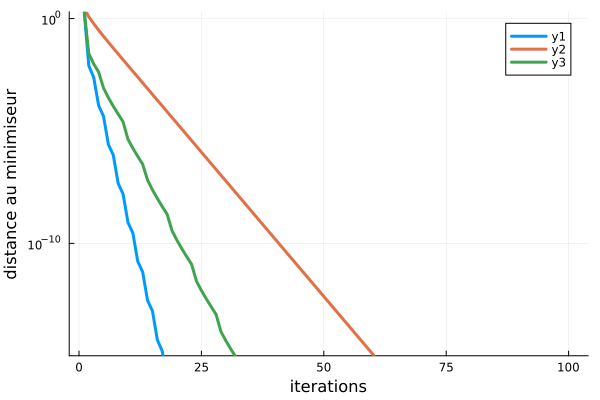
\includegraphics[width=0.4\textwidth]{exemple-steps}
		\caption{Descente de gradient}
		\label{fig:cv}
	\end{figure}
	
	\item Les factorisations suivantes sont-elles des décompositions en valeurs singulières? Justifier dans chaque cas.
	
	\hspace{-12mm}
	\begin{tabular}{ll}
		 (a) $\displaystyle A = \begin{bmatrix} \frac{1}{\sqrt{2}} & 0 \\ \frac{1}{\sqrt{2}} & 1 \end{bmatrix} \begin{bmatrix} 5 & 0 \\ 0 & 2 \end{bmatrix} \begin{bmatrix} 0 & 1  \\ 1 & 0  \end{bmatrix}$
		& 
		(b) $\displaystyle B = \begin{bmatrix} \frac{1}{\sqrt{2}} & -\frac{1}{\sqrt{2}} \\ \frac{1}{\sqrt{2}} & \frac{1}{\sqrt{2}} \end{bmatrix} \begin{bmatrix} 3 & 0 & 0\\ 0 & 1 & 0 \end{bmatrix} \begin{bmatrix} \frac{1}{\sqrt{2}} & 0 & \frac{1}{\sqrt{2}} \\ 0 & 1 & 0 \\ \frac{1}{\sqrt{2}} & 0 & -\frac{1}{\sqrt{2}} \end{bmatrix}$
		\\		
		\\
		(c) $\displaystyle C = \begin{bmatrix} 1 & 0 & 0 \\ 0 & 1 & 0 \\ 0 & 0 & 1 \end{bmatrix} \begin{bmatrix} 1 & 0\\ 0 & -1 \\ 0 & 0\end{bmatrix} \begin{bmatrix} \frac{1}{\sqrt{2}} & -\frac{1}{\sqrt{2}} \\ \frac{1}{\sqrt{2}} & \frac{1}{\sqrt{2}} \end{bmatrix}$
		&
		(d) $\displaystyle D = \begin{bmatrix} 1 & 2 \\ -1 & 2 \end{bmatrix} \begin{bmatrix} 3 & 0 \\ 0 & 0 \end{bmatrix} \begin{bmatrix} 1 & -1 \\ 1 & 1\end{bmatrix}$.
	\end{tabular}
	
	\item On considère le réseau à deux couches représenté en Figure~\ref{fig:nn}, 
où l'on a explicitement représenté la fonction non-linéaire $\sigma$ et les biais $b_1$, $b_2$:
	\begin{figure}[h!]
	\centering
	\begin{tikzpicture}
		\node[circle,fill,inner sep=2pt,label=left:$x_1$](x1){};
		\node[circle,fill,inner sep=2pt,label=left:$x_2$,below=2cm of x1](x2){};
		\node[circle,fill,inner sep=2pt,label=left:$x_3$,below=2cm of x2](x3){};
		
		\node[circle,fill,inner sep=2pt,label=above:$z_1$,above right=1cm and 3.5cm of x2](h1){};
		\node[circle,fill,inner sep=2pt,label=below:$z_2$,below=2cm of h1](h2){};
		
		\node[above right=5mm and 2.5cm of x1,circle,fill,inner sep=2pt,label=above:$1$](b1){};
		\node[below right=5mm and 2.5cm of x3,circle,fill,inner sep=2pt,label=below:$1$](b2){};
		
		\draw[orange] (x1) -- node[above]{$w_{11}$} (h1);
		\draw[orange] (x2) -- node[above]{$w_{12}$} (h1);
		\draw[orange] (x3) -- node[above]{$w_{13}$} (h1);
		
		\draw[blue] (x1) -- node[below,near start,xshift=-2mm]{$w_{21}$} (h2);
		\draw[blue] (x2) -- node[below,near start]{$w_{22}$} (h2);
		\draw[blue] (x3) -- node[below]{$w_{23}$} (h2);
		
		\draw[dashed] (b1) -- node[above,xshift=1mm]{$b_1$} (h1);
		\draw[dashed] (b2) -- node[below,xshift=1mm]{$b_2$} (h2);
		

		\node[circle,fill,inner sep=2pt,right=2.5cm of h1] (z1) {};
		\node[circle,fill,inner sep=2pt,right=2.5cm of h2] (z2) {};
		
		\draw[dashed]  (h1) -- (z1);
		\draw[dashed]  (h2) -- (z2);
		\path[] (h1) -- node[draw,fill=white]{$\sigma$} (z1);
		\path[] (h2) -- node[draw,fill=white]{$\sigma$} (z2);
		
		\node[circle,fill,inner sep=2pt,below right= 1cm and 2.5cm of z1,label=right:$y$] (o) {};
		
		\draw[] (z1) -- node[above]{$v_{1}$} (o);
		\draw[] (z2) -- node[above]{$v_{2}$} (o);

		

		
		%\node[below right = -15pt and 5cm of h2] {$\displaystyle y = \sum_{k=1}^n v_k \, \sigma(\ww_k^\top \xx+b_k)$};
	\end{tikzpicture}
	\caption{Réseau de neurones}
	\label{fig:nn}
	\end{figure}
%

	\begin{enumerate}
	\item Exprimer les sorties intermédiaires $z_1$ et $z_2$ en fonction de l'entrée $\mathbf{x} = \begin{bmatrix} x_1 & x_2 & x_3\end{bmatrix}^\top$ des vecteurs de poids $\mathbf{w_1} = \begin{bmatrix} w_{11} & w_{12} & w_{13} \end{bmatrix}^\top$, $\mathbf{w_2} = \begin{bmatrix} w_{21} & w_{22} & w_{23} \end{bmatrix}^\top$, et des biais $b_1$, $b_2$.
	\item  Exprimer de même la sortie finale $y$ en fonction de $\mathbf{x}$ et des différents paramètres du réseau.
	\end{enumerate}
\end{enumerate}


\section{Optimisation numérique}

%On considère la fonction de trois variables suivantes
%\eq{
%	f(x_1,x_2,x_3) = x_1^2 - 2x_1x_2 + x_2^2 - 2x_2x_3 + 2x_3^2 + 2x_1x_3 - 4x_3 + 5
%}

\label{sec:mc}
On considère un vecteur $\mathbf{x}_0 \in \RR^3$ inconnu, et des observations $\mathbf{y}\in\RR^3$ de la forme
\eq{
	\mathbf{y} = \mathbf{A}\mathbf{x}_0 + \bm{\eps}, \quad \mathbf{A} = \begin{bmatrix} 1 & -1 & 1 \\ -1 & 1 & -1 \\ 1 & -1 & -2 \end{bmatrix}
}
où $\bm{\eps} \in \RR^3$ modélise les erreurs de mesures. On souhaite estimer $\mathbf{x}_0$ à partir de $\mathbf{y}$ en résolvant le problème des moindres carrés
\eql{\label{eq:mc}
	\min_{\mathbf{x}\in\RR^3} \frac{1}{2}\norm{\mathbf{A}\mathbf{x} -\mathbf{y}}_2^2
}
où $\norm{\cdot}_2$ est la norme euclidienne usuelle.

\begin{enumerate}
	%\item %On cherche à estimer $\mathbf{x}$ à partir de $\mathbf{y}$ au sens des moindres carrés. Ecrire le problème d'optimisation correspondant.
	%\eq{
	%	\min_{\mathbf{x}\in\RR^3} f(\mathbf{x})
	%}
%	\item Exprimer $f$ sous la forme
%	\eq{
%		f(x_1,x_2,x_3) = \frac{1}{2}\mathbf{x}^\top \mathbf{Q}\mathbf{x} + \mathbf{q}^\top \mathbf{x} + r
%	}
%	en explicitant les différentes quantités.

	\item Ce problème admet-il un minimiseur unique? pas de minimiseur? plusieurs minimiseurs? Justifier votre réponse.
	
	\item On considère le critère régularisé
	\eq{
		f(\mathbf{x}) \eqdef \frac{1}{2}\norm{\mathbf{A}\mathbf{x} - \mathbf{y}}_2^2 + \frac{1}{2} \norm{\mathbf{x}}_2^2.
	}
	Montrer que $f(\mathbf{x})$ peut s'écrire sous la forme
	\eq{
		\frac{1}{2}\mathbf{x}^\top \mathbf{P} \mathbf{x} + \mathbf{q}^\top \mathbf{x} + r
	}
	où vous expliciterez $\mathbf{P}$, $\mathbf{q}$ et $r$.
	%Exprimer $f(\mathbf{x})$ sous la forme
	%$
	%	\frac{1}{2}\mathbf{x}^\top \mathbf{Q}\mathbf{x} + \mathbf{q}^\top \mathbf{x}
	%$
	%en explicitant les différentes quantités.
	
	\item En détaillant les calculs, exprimer le gradient $\nabla f(\mathbf{x})$ en fonction de $\mathbf{A}$ et $\mathbf{y}$.
	
	\item En expliquant votre démarche, exprimer la solution du problème d'optimisation
	\eq{
		\min_{\mathbf{x} \in \RR^3} f(\mathbf{x})
	}
	en fonction de $\mathbf{A}$ et $\mathbf{y}$.
	%\todo{Calcul pour $\lambda$ et inverse donné?}
	
\end{enumerate}

\section{Classification}

\subsection{Séparateur linéaire}
On considère un jeu de données constitué de $8$ échantillons dans $\RR^2$, labellisés positivement et négativement:
	\begin{itemize}
		\item[-] classe $+1$ : $(1,2)$, $(3/2,3)$, $(3,2)$, $(3,4)$
		\item[-] classe $-1$ : $(1,0)$, $(2,1)$, $(3,0)$, $(2,-1)$
	\end{itemize}
	
\begin{enumerate}
	\item Représenter les observations sur la Figure \ref{fig:jeu-1} en utilisant 2 couleurs (ou 2 formes) différentes pour distinguer les classes.
	\item Représenter l'hyperplan optimal au sens des SVM. Donner son équation et calculer sa marge.
	\item Quels sont les vecteurs de support?
\end{enumerate}

\subsection{Astuce du noyau}
On considère un nouveau jeu de données, constitué de $4$ échantillons étiquetés positivement: $(2,2)$, $(2,-2)$, $(-2,-2)$, $(-2,2)$ et $4$ échantillons étiquetés négativement: $(1,1)$, $(1,-1)$, $(-1,-1)$, $(-1,1)$.

\begin{enumerate}
	\item Représenter ces observations sur la Figure \ref{fig:jeu-2} avec deux couleurs différentes. Les classes sont-elles linéairement séparables?
	
	\item Expliquer en quelques lignes le principe de l'astuce du noyau.
	
	\item On considère la fonction de redescription suivante:
	\eq{
		\phi(\mathbf{x}) = \left\{\begin{array}{ll}
			(4-x_2 + \abs{x_1-x_2} + 1, 4-x_1 + \abs{x_1-x_2} + 1) &\text{si}\;\; \norm{x}_2 > 2\\
			(x_1,x_2) &\text{sinon}
			\end{array}\right.
	}
	Calculer les coordonnées des échantillons dans l'espace de redescription et les représenter en Figure \ref{fig:jeu-t} en utilisant les mêmes couleurs qu'en 1.
	
	\item Tracer sur la même figure l'hyperplan optimal au sens des SVM, donner son équation et calculer sa marge.
	
	\item Quelle est la classe attribuée à un échantillon de coordonnée $(6,6)$ dans l'espace d'origine?
	
	\item Donner un exemple d'une autre fonction de redescription $\psi : \RR^2 \to \RR^3$ qui aurait pu être utilisée pour classifier ces données.
\end{enumerate}

\begin{figure}[h!]
\centering
\subfloat[Jeu n°1\label{fig:jeu-1}]{
\begin{tikzpicture}

\draw[step=0.5,gray] (-1,-2) grid (5,4);


\node at (-1.5,-1) {-1};
\node at (-1.5,0) {0};
\node at (-1.5,1) {1};
\node at (-1.5,2) {2};
\node at (-1.5,3) {3};

\draw[-latex,thick] (-1,0) -- (5,0);
\draw[-latex,thick] (0,-2) -- (0,4);

\node at (0,-2.5) {0};
\node at (1,-2.5) {1};
\node at (2,-2.5) {2};
\node at (3,-2.5) {3};
\node at (4,-2.5) {4};

\end{tikzpicture}
}
%
\subfloat[Jeu n°2\label{fig:jeu-2}]{
\begin{tikzpicture}

\draw[step=0.5,gray] (-3,-3) grid (3,3);


\node at (-3.5,-2) {-2};
\node at (-3.5,-1) {-1};
\node at (-3.5,0) {0};
\node at (-3.5,1) {1};
\node at (-3.5,2) {2};

\draw[-latex,thick] (-3,0) -- (3,0);
\draw[-latex,thick] (0,-3) -- (0,3);


\node at (-2,-3.5) {-2};
\node at (-1,-3.5) {-1};
\node at (0,-3.5) {0};
\node at (1,-3.5) {1};
\node at (2,-3.5) {2};

\end{tikzpicture}
}

\subfloat[Jeu n°2 - redescription\label{fig:jeu-t}]{
\begin{tikzpicture}

\draw[step=0.5,gray] (-1,-1) grid (6,6);


\node at (-1.5,0) {0};
\node at (-1.5,1) {2};
\node at (-1.5,2) {4};
\node at (-1.5,3) {6};
\node at (-1.5,4) {8};
\node at (-1.5,5) {10};

\draw[-latex,thick] (-1,0) -- (6,0);
\draw[-latex,thick] (0,-1) -- (0,6);


\node at (0,-1.5) {0};
\node at (1,-1.5) {2};
\node at (2,-1.5) {4};
\node at (3,-1.5) {6};
\node at (4,-1.5) {8};
\node at (5,-1.5) {10};

\end{tikzpicture}
}
\caption{Classification}
\end{figure}



\section{Décompositions matricielles}
\begin{enumerate}
	
	
	
	\item On considère dans cette question la matrice $\mathbf{A}$ définie dans l'exercice \ref{sec:mc} ci-dessus.
	\begin{enumerate}
		\item Calculer la matrice $\mathbf{B} = \mathbf{A}^\top \mathbf{A}$.
		\item Quel est le rang de $\mathbf{B}$? En déduire une valeur propre et un vecteur propre de $\mathbf{B}$ (on rappelle qu'un couple valeur/vecteur propre est un couple $(\lambda,\mathbf{v})$ tel que $\mathbf{v}\neq 0$ et $\mathbf{B}\mathbf{v} = \lambda \mathbf{v}$).
		\item Quel est le rang de $\mathbf{B}-6\mathbf{I}_3$? Trouver deux vecteurs $\mathbf{v}_1,\mathbf{v}_2 \in \RR^3$ non colinéaires (et non nuls) tels que $\mathbf{B}\mathbf{v}_1=6\mathbf{v}_1$ et $\mathbf{B}\mathbf{v}_2=6\mathbf{v}_2$.
		\item Trouver les valeurs singulières de $\mathbf{A}$, ainsi que les vecteurs singuliers droits associés.
	\end{enumerate}
	
	\item Soit $\mathbf{X} \in \RR^{m\times n}$, pour $m,n \in \NN$ donnés. On note
	\eq{
		\mathbf{X} = \mathbf{U}\diag(\sigma_1,\ldots,\sigma_r,0,\ldots,0)\mathbf{V}^\top
	}
	la décomposition en valeurs singulières de $\mathbf{X}$, avec $\sigma_1 \geq \ldots \geq \sigma_r > 0$. Montrer que \eq{\norm{X}_F = \sqrt{\sum_{j=1}^r \sigma_j^2}} où $\norm{\mathbf{X}}_F = \sqrt{\Tr(\mathbf{X}^\top \mathbf{X})}$ est la norme de Frobenius.
	
	%\noindent \textbf{Indication}: On rappelle que $\Tr(AB) = \Tr(BA)$ pour toutes matrices $A$, $B$ (de tailles compatibles).
\end{enumerate}
 
\end{document}
